%%%%%%%%%%%%%%%%%%%%%%%%%%%%%%%%%%%%%%%%%%%%%%%%%%%%%%%%%%%%%%%%%%%%
\section{Organization and Management}
\label{sec:fdsp-pd-org}
%\metainfo{\color{red}\bf  Content: Segreto/Warner}

The single-phase photon detector consortium has and will continue to benefit from the contributions of many institutions and facilities in Europe and North and South America.  Tables~\ref{tab:sp-pds-institutes-i} and \ref{tab:sp-pds-institutes-ii} list the member institutions. 
%To help guide the interactions of these many contributors, the consortium is divided into six working groups, each with two or three conveners, to direct its activities.  % The structure of the organization is detailed below.

%%%%%%%%%%%%%%%%%%%%%%%%%%%%%%%%%%%
%\subsection{Consortium Organization}
\label{sec:fdsp-pd-org-consortium}
%\fixme{Please remove org chart with names and add a list of institutions. Template provided. Anne 4/16}
%\fixme{Dave/Ettore: Table needs completing. The org chart needs to be commented out and the text changed to refer to the new table.}

\begin{dunetable}
[PDS Consortium Institutions - Part I]
{ll}
{tab:sp-pds-institutes-i}
{PDS Consortium Institutions - Part I}
Member Institute         &  Country       \\  \colhline
Federal University of ABC & Brazil \\ \colhline
State University of Feira de Santana & Brazil \\ \colhline
Federal University of Alfenas Po\c{c}os de Caldas & Brazil \\ \colhline
Centro Brasileiro de Pesquisas Físicas & Brazil \\ \colhline
Federal UNiversity de Goias & Brazil \\ \colhline
Brazilian Synchotron Light Laboratory LNLS/CNPEM & Brazil \\ \colhline
Sate University of Campinas & Brazil \\ \colhline
CTI Renato Archer & Brazil \\ \colhline
Federeal Technological University of Paran\'a & Brazil \\ \colhline
Universidad del Atlantico & Colombia \\ \colhline
Universidad Sergia Ablada & Colombia \\ \colhline
University Antonio Nari\~{n}o & Colombia \\ \colhline
Institute of Physics CAS & Czech Republic \\ \colhline
Czech Technical University in Prague & Czech Republic \\ \colhline
Universidad Nacional de Assuncion & Paraguay \\ \colhline
Pontificia Universidad Catilica Per\'{u} & Per\'{u} \\ \colhline
Universidad Nacional de Ingineria & Per\'{u} \\ \colhline
University of Warwick & UK \\ \colhline
University of Sussex & UK \\ \colhline
University of Manchester & UK \\ \colhline
Edinburgh University & UK \\ \colhline
Argonne National Laboratory & UK \\\colhline
Brookhaven National Laboratory & UK \\ \colhline
California Institute of Technology & UK \\ \colhline
Colorado State University   &  USA  \\ \colhline
\dword{fnal}    &   USA    \\ \colhline
Duke University & USA \\ \colhline
Idaho State University & USA \\ \colhline
Indiana University & USA \\ \colhline
University of Iowa & USA \\ \colhline
Louisiana State University & USA \\ \colhline
Massachusetts Institute of Technology & USA \\ \colhline
University of Michigan & USA \\ \colhline
Northern Illinois University & USA \\ \colhline
South Dakota School of Mines and Technology & USA \\ \colhline
Syracuse University & USA \\ \colhline
University of Bologna and INFN & Italy \\ \colhline
University of Milano Bicocca and INFN & Italy \\ \colhline
\end{dunetable}

\begin{dunetable}
[PDS Consortium Institutions - Part II]
{ll}
{tab:sp-pds-institutes-ii}
{PDS Consortium Institutions - Part II}
Member Institute         &  Country       \\  \colhline
University of Genova and INFN & Italy \\ \colhline
University of Catania and INFN & Italy \\ \colhline
Laboratori Nazionali del Sud & Italy \\ \colhline
University of Lecce and INFN & Italy \\ \colhline
INFN Milano & Italy \\ \colhline
INFN Padova & Italy \\ 
\end{dunetable}


The \single \dword{pds} consortium follows the typical organizational structure of DUNE consortia:
\begin{itemize}
\item A Consortium Lead provides overall leadership for the effort, and attends meetings of the DUNE Executive and Technical Boards.
\item A Technical Lead provides technical support to the consortium lead, attends the Technical Board and other project meetings, oversees the project schedule and \dword{wbs}, and oversees the operation of the project working groups.  
%In the case of the \dword{pds}, the technical lead is supported by a deputy technical lead.
\end{itemize}

%\begin{dunefigure}[PDS consortium organization chart]{fig:pds-org-chart}
%{\dword{pds} consortium organization chart.}

%	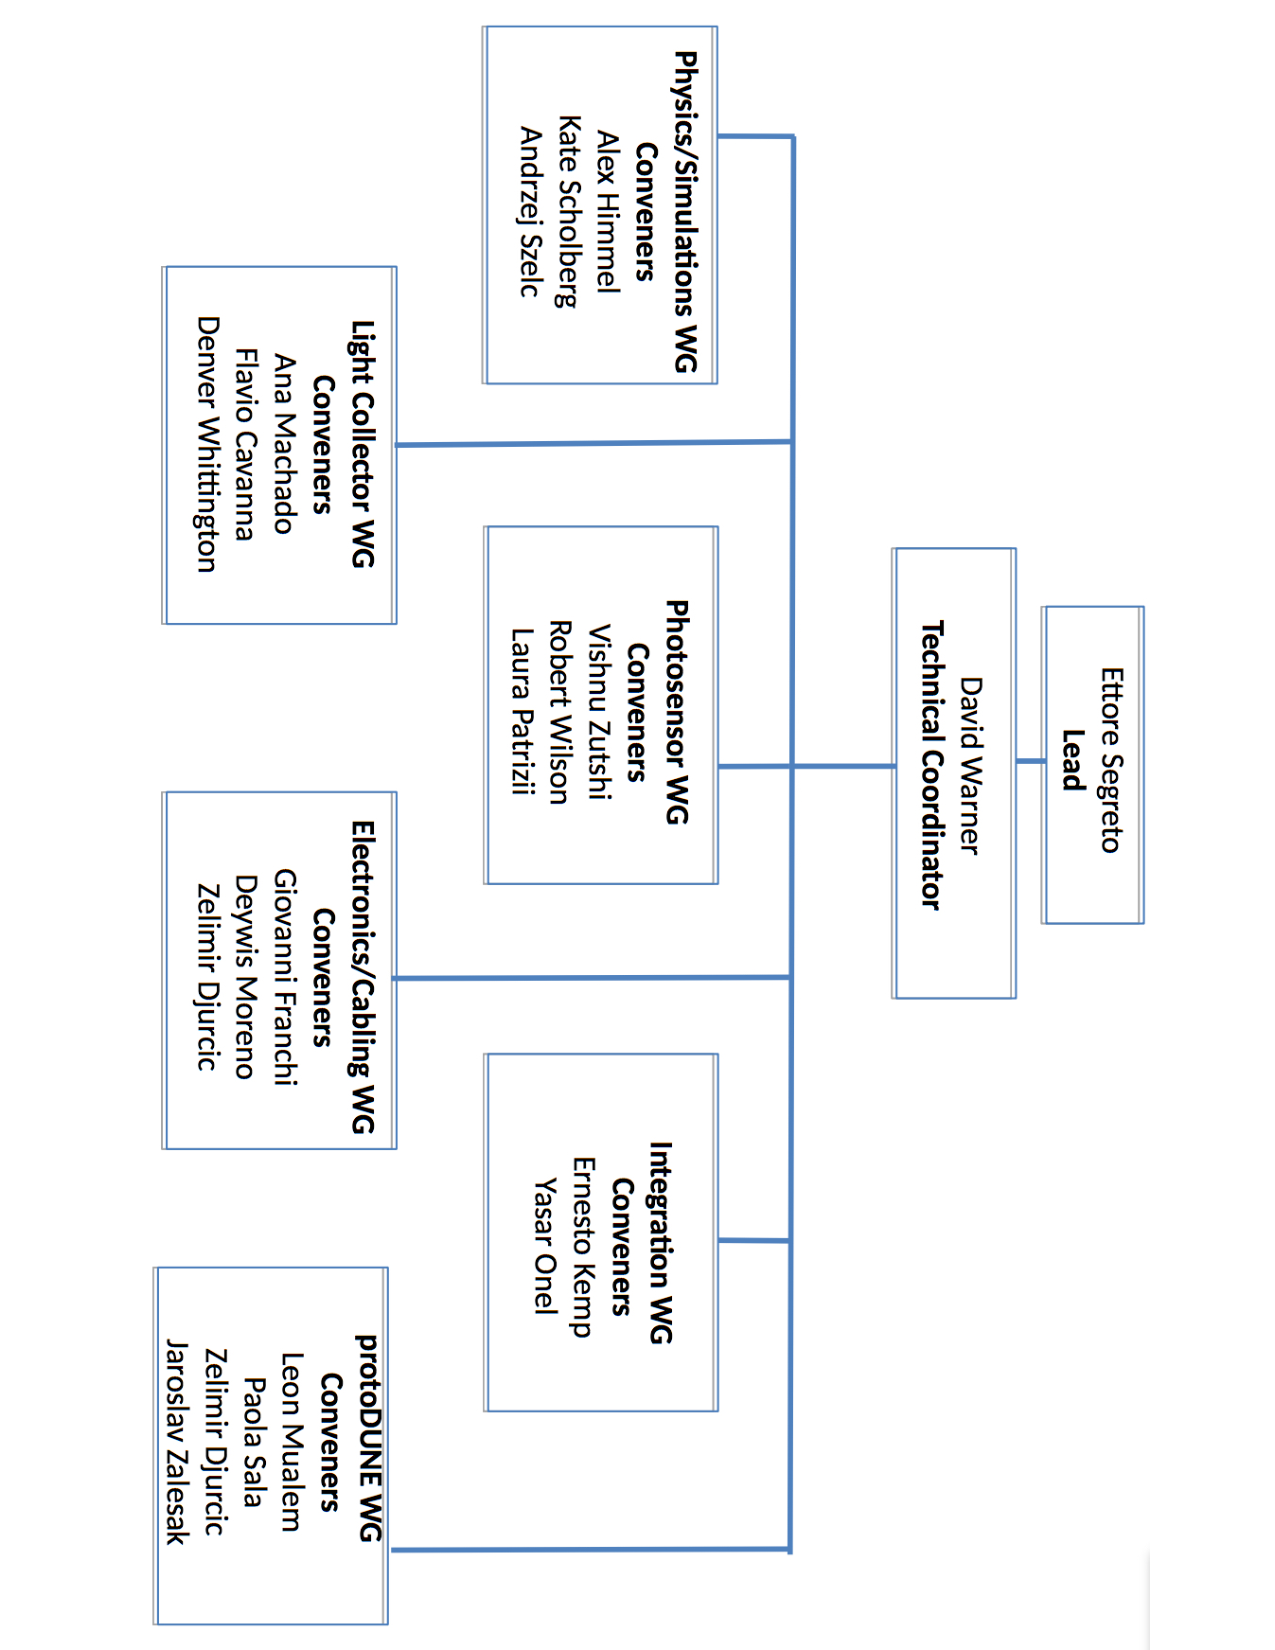
\includegraphics[angle=90,height=12cm]{pds-consortium-org-chart}
	
%\end{dunefigure} 

Below the leadership, the consortium is divided up into six working groups, each led by two or three working group conveners.  Each working group is charged with one primary area of responsibility within the consortium, and the conveners report directly to the technical lead regarding those responsibilities. %As the consortium advances to a more detailed \dword{wbs} and project schedule, it is envisioned that each working group will be responsible for one section of those documents.

The working group conveners are appointed by the \dword{pds} Consortium Lead and Technical Lead; the structure may evolve as the consortium matures and additional needs are identified. 

%%%%%%%%%%%%%%%%%%%%%%%%%%%%%%%%%%
%\subsection{Project Planning Assumptions}
%\label{sec:fdsp-pd-org-assmp}

%\fixme{I think this sub-section is redundant and can be removed.  It is all still here if you want to resurrect it.}
%\metainfo{\color{blue} Content: Segreto/Warner}

%Plans for the \dword{pds} consortium are based on the overall schedule for the DUNE \dword{fd}. In particular, the \dword{apa} schedule defines the time window for the completion of the final development program for the light collectors: A final down-select to a baseline light collector option and \dword{fe} electronics has been made for the TDR.  Due to the opportunities presented by our new Italian colleagues and their close connection with FBK, we may maintain an alternate photosensor option up to the pre-production review in September of 2020, but all other systems must be defined prior to the \dword{tdr}.

%The \dword{pds} modules will undergo final assembly and testing at the \dword{pds} assembly facility at UNICAMP, with an initial  assembly rate of approximately twenty modules per week, accelerating to forty modules per week in the second half of module fabrication.  

%The modules will be shipped from the fabrication facilities to the project storage facility, 
%to be integrated along with the \dword{ce} into the \dword{apa} frames and cold tested in a cryogenic test facility.  We plan for an initial rate of two \dwords{apa} per week, with the possibility of accelerating to four \dwords{apa} per week as production lessons are learned.  \Dword{pds} personnel will be present at the integration facility to oversee the installation and testing.

%Meeting this timeline requires that the development of the ARAPUCA system be aggressively pursued throughout 2018, with a goal of testing near-final prototypes in the late fall of 2018 and allowing technology comparisons between the ARAPUCA and the light guide technologies in winter of 2019.

%Additional development efforts will focus on:

%\begin{itemize}
%\item identifying and selecting reliable cryogenic photosensor (\dword{sipm}) candidates,
%\item reducing cost and optimizing performance of \dword{fe} electronics, and 
%\item solidifying \dword{pds} performance requirements from additional physics simulation efforts.
%\end{itemize}

%We assume that apart from these items, where rapid development is still required, most of the detector components to be delivered by the \dword{pd} consortium will require only minor changes relative to the \dword{pdsp} components. For this reason, modifications of these other detector components will be delayed until 2019, which will also help with the funding profile. Exceptions will be made for further development in test stands with regard to cabling studies, and for the interface engineering required to ensure satisfactory integration of the \dword{pd} with the \dword{apa} and \dword{ce}  systems.

%%%%%%%%%%%%%%%%%%%%%%%%%%%%%%%%%%%
%\subsection{WBS and Responsibilities}
%\label{sec:fdsp-pd-org-wbs}
%\metainfo{\color{blue} Content: Warner/Mualem}

%%%%%%%%%%%%%%%%%%%%%%%%%%%%%%%%%%
\subsection{High-Level Schedule}
\label{sec:fdsp-pd-org-cs}

\forlbnc{LBNC:  This section is a placeholder.  Milestones of \dword{pd} system development and fabrication are shown in order, however the integrated project schedule is still being developed and no dates are shown at this time.  The correct schedule milestone dates will be inserted into the final revision to be presented in July.}


%\fixme{This is a standard table template for the TDR schedules.  It contains overall FD dates from Eric James as of March 2019 (orange) that are held in macros in the common/defs.tex file so that the TDR team can change them if needed. Please do not edit these lines! Please add your milestone dates to fit in with the overall FD schedule. And fix table captions and label, please. (Anne)}


\begin{dunetable}
[PDS Consortium Schedule]
{p{0.65\textwidth}p{0.25\textwidth}}
{tab:Xsched}
{PDS Consortium Schedule}   
Milestone & Date (Month YYYY)   \\ \toprowrule
60 percent design review &      \\ \colhline
Final design review for PD rails, cables, connectors & \\ \colhline
\dword{prr} for PD rails, cables. connectors & \\ \colhline
Fabrication of PD rails, cables, connectors begins &  \\ \colhline
Down selection to two photosensor candidates &      \\ \colhline
Final design review for remaining PD components &      \\ \colhline
Start of module 0 component production for ProtoDUNE-II &      \\ \colhline
End of module 0 component production for ProtoDUNE-II &      \\ \colhline
\rowcolor{dunepeach} Start of \dword{pdsp}-II installation& \startpduneiispinstall      \\ \colhline
\dword{prr} for photosensors &      \\ \colhline
Begin procurement of photosensors  &      \\ \colhline
Start of \dword{pdsp}-II operations &      \\ \colhline
\dword{prr} for remaining photon detector components &      \\ \colhline
\rowcolor{dunepeach} Start of \dword{pddp}-II installation& \startpduneiidpinstall      \\ \colhline
Begin procurement of filter plates  &      \\ \colhline
Begin fabrication/procurement of remaining module components  &      \\ \colhline
Begin assembly of X-ARAPUCA modules  &      \\ \colhline
Begin assembly of front-end electronics modules  &      \\ \colhline
Begin assembly of PD monitoring system  &      \\ \colhline
\rowcolor{dunepeach}South Dakota Logistics Warehouse available& \sdlwavailable      \\ \colhline
\rowcolor{dunepeach}Beneficial occupancy of cavern 1 and \dword{cuc}& \cucbenocc      \\ \colhline
(\#1 TPC) First 500 modules at Logistics Warehouse   &    \\ \colhline
\rowcolor{dunepeach} \dword{cuc} counting room accessible& \accesscuccountrm      \\ \colhline
\rowcolor{dunepeach}Top of \dword{detmodule} \#1 cryostat accessible& \accesstopfirstcryo      \\ \colhline
(\#1 TPC) Remaining 1000 modules at Logistics Warehouse   &    \\ \colhline
(\#1 TPC) Front end electronics modules at Logistics Warehouse   &    \\ \colhline
\dword{pd} monitoring system at Logistics Warehouse   &    \\ \colhline
\rowcolor{dunepeach}Start of \dword{detmodule} \#1 TPC installation& \startfirsttpcinstall      \\ \colhline
\rowcolor{dunepeach}End of \dword{detmodule} \#1 TPC installation& \firsttpcinstallend      \\ \colhline
\rowcolor{dunepeach}Top of \dword{detmodule} \#2 accessible& \accesstopsecondcryo      \\ \colhline
(\#2 TPC) \dword{pd} light collector modules at Logistics Warehouse   &    \\ \colhline
(\#2 TPC) Remaining 1000 modules at Logistics Warehouse   &    \\ \colhline
(\#2 TPC) Front end electronics modules at Logistics Warehouse   &    \\ \colhline
 \rowcolor{dunepeach}Start of \dword{detmodule} \#2 TPC installation& \startsecondtpcinstall      \\ \colhline
\rowcolor{dunepeach}End of \dword{detmodule} \#2 TPC installation& \secondtpcinstallend      \\ \colhline

\end{dunetable}



%The high-level schedule for the photon detector consortium through submission of the \dword{tdr} at the end of Q2 in FY19 is detailed in Figure~\ref{fig:pds-sched-to-tdr} and the pre-\dword{tdr} key milestones are listed in Table~\ref{fig:pds-pretdrkeymilestones}.

%\begin{dunefigure}[\dword{pd}S consortium schedule through to the \dword{tdr}.]{fig:pds-sched-to-tdr}
%{Photon Detector System consortium schedule through to the \dword{tdr}.}
 %%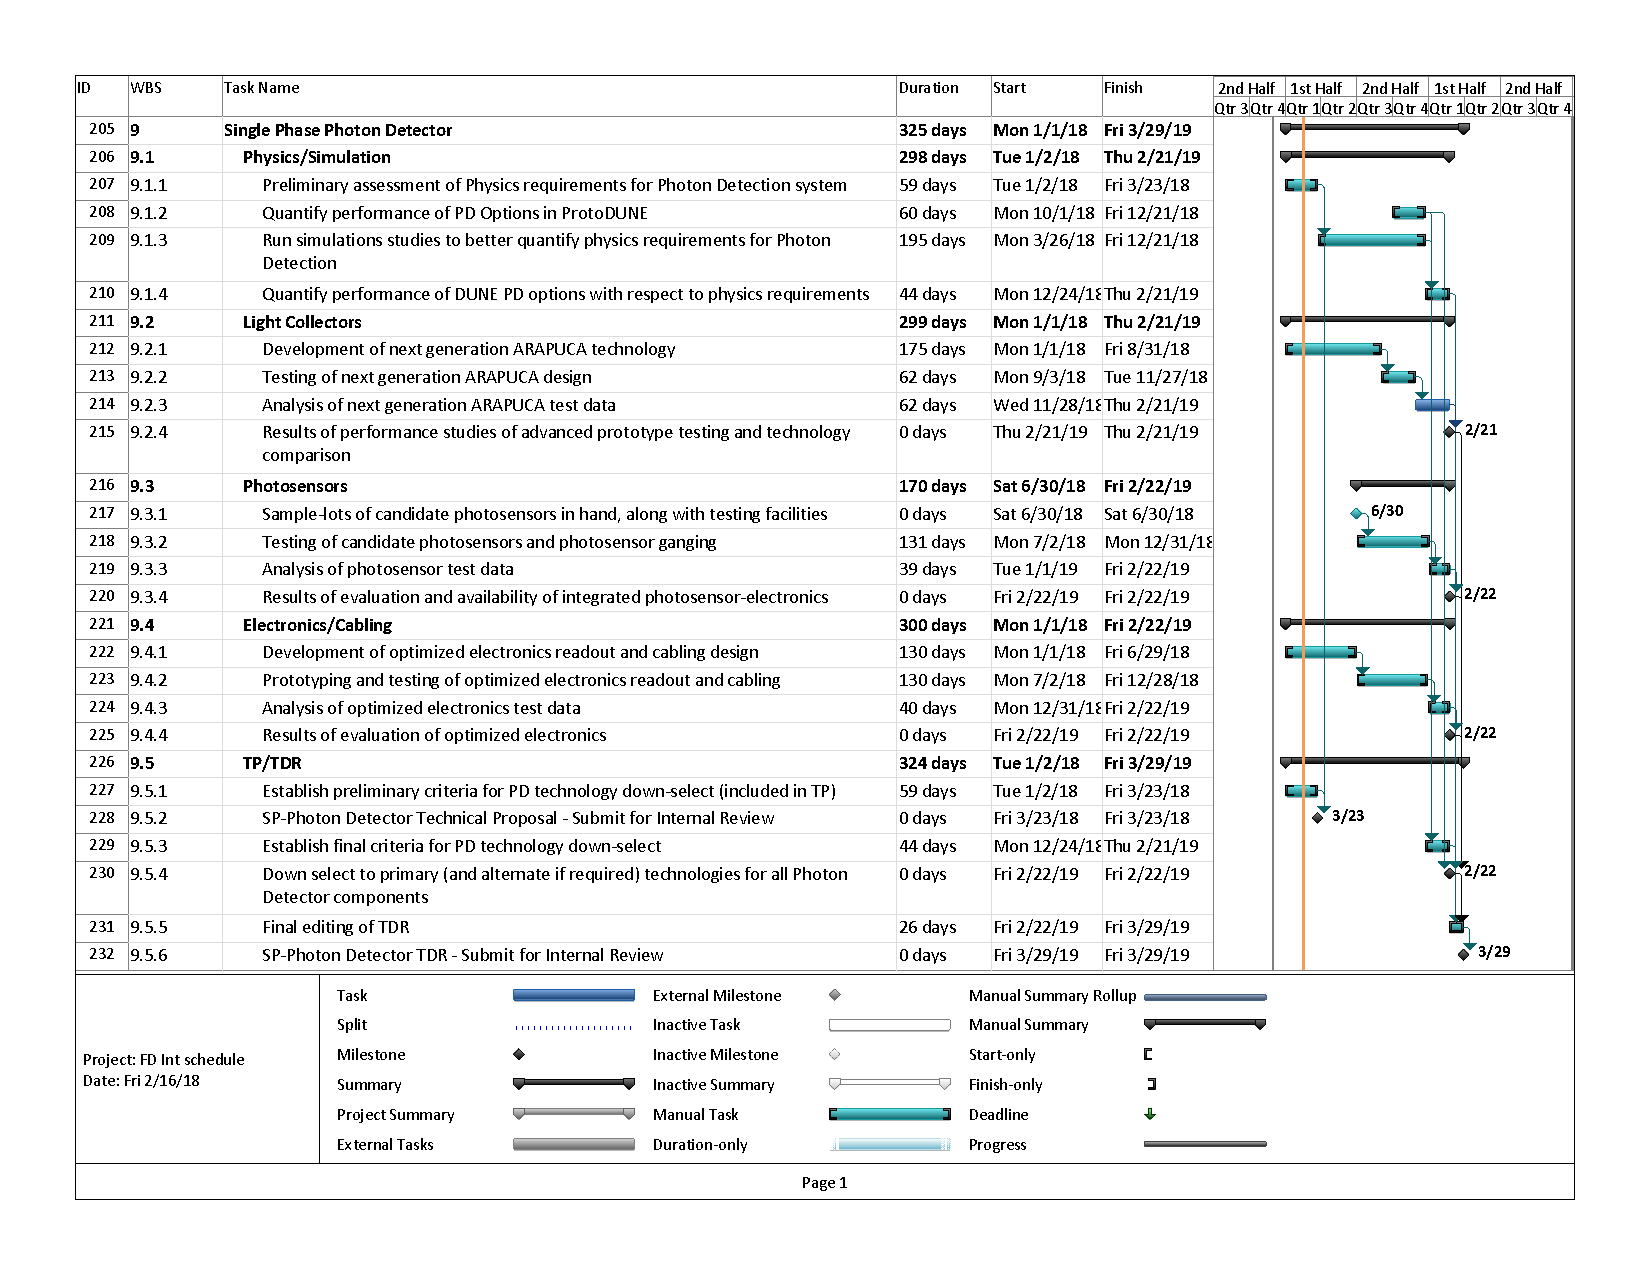
\includegraphics[width=1.0\columnwidth]{pds-sched-to-tdr.pdf}
%\end{dunefigure}

%\fixme{Dave W:  Will be updated in March 2019 per Eric.} Is on Dave's todo list. Comment added to the caption.

%\fixme{DWW: will replace milestone tables.}

%\begin{dunetable}[Pre-\dword{tdr} key milestones. Will be updated in March 2019.]
%{ll}
%{fig:pds-pretdrkeymilestones}
%{Pre-\dword{tdr} key milestones. Will be updated in March 2019.}
%Milestone													&	Date	       \\ \toprowrule
%Preliminary \dword{pd} technology selection criteria determined				&	03/21/18	\\ \colhline
%Results from final prototype light collector studies available			&	02/21/19	\\ \colhline
%Final \dword{pd} technology selection criteria available						&	02/21/19	\\ \colhline
%Down-select to primary (and potential alternate) light collector technology	&	02/22/19	\\ \colhline
%Submit initial \dword{tdr} draft for internal review							&	03/29/19	\\ 
%\end{dunetable}

%High-level post-\dword{tdr} milestones are listed in Table~\ref{fig:pds-posttdrkeymilestones}.

%LMM fixed detector -> Module below and 10 kt -> \SI{10}{kt}

%\begin{dunetable}[Post-\dword{tdr} key milestones.]
%{ll}
%{fig:pds-posttdrkeymilestones}
%{Post-\dword{tdr} key milestones.}
%Milestone											&	Date	       \\ \toprowrule
%\dword{pd} pre-production review(s) complete					&	03/2020 	\\ \colhline
%Initial \dword{pd} module fabrication begins						&	09/2020	\\ \colhline
%Final \dword{pd} production review based on initial production \dword{qa}		&	02/2021	\\ \colhline
%First  \dword{pd} modules delivered for installation				&	05/2021	\\ \colhline
%Installation into \dwords{apa} begins							&	06/2021     \\ \colhline
%\dword{pd} fabrication complete (first \dword{spmod})			&	07/2023	\\ 
%\end{dunetable}

\subsection{High-Level Cost Summary}

%\fixme{New cost table template to come early April. Anne}

\forlbnc{Note to reviewers:  This section is a placeholder - costs will be inserted prior to submission of the final revision in July.}

In the fall of 2018 we completed an initial cost estimate for fabrication of \dword{pd} modules for one 10kt \dword{dune} detector.  The estimates were based on ProtoDUNE costs, modified as necessary for an \dword{xarapu} design.  Vendor quotations were used for most of the major components.  The biggest uncertainties in fabrication costs center around the photosensor fabrication, which currently constitute approximately half the total PD system cost.  We have estimates from Hamamatsu for photosensors which would reduce this line by nearly a factor of two, significantly reducing the system cost.  We also have preliminary indications that similar cost savings may also be available from using FBK photosensors.  As noted earlier in this \dword{tdr}, a major focus of our remaining development work centers is focused on realizing these potential savings.

The dichroic filter procurement and coating represent the other major cost driver for the project.  The costing for the filter plates is based on initial contacts with a Brazilian filter firm, but samples of these filters were recently procured and we are currently awaiting results from coating tests.   These filter plates are very significantly cheaper than the filters manufactured by Omega Inc. and tested in our earlier validation studies.  Until these tests are complete, the filter plates remain a significant cost and schedule risk.

%\fixme{DWW: will update previous paragraph.}

%\fixme {DWW: Placeholder numbers (DWW)  NOT ACCURATEcurrently in table.  Will update in April 2019} Comment added to the caption.
\begin{dunetable}
[Single Phase Photon detector System Cost Summary.]
{p{0.7\textwidth}p{0.2\textwidth}}
{tbl:sppdcostsumm}
{Single Phase Photon Detector System Cost Summary. Will update prior to TDR submission in July.}
Item & Core Cost (k\$ US) \\ \toprowrule
Design, Engineering and Development & \num{1.0} \\ \colhline
Production Setup & \num{1.0} \\ \colhline
Production & \num{1.0} \\ \colhline
Integration & \num{1.0}\\ \colhline
Installation & \num{1.0} \\ 

\end{dunetable}

%\fixme{Anne--  will there be a standard table for the labor as well?}

%\fixme{Stolen from CE!  Need to change to pd-specific!DWW:  Labor placeholder table.  Will update in April 2019. }; on Dave's todo list. Comment added to the caption.
%\fixme{Anne:  I believe you will paste in new cos tables here, right?}

%\begin{dunetable}
%[Personnel needs for the \dword{pd} consortium. Will update prior to TDR submission in July.]
%{lrrrrr}
%{tab:SPCE:personnel}
%{Personnel needs (in FTE--years) for the construction of the \dword{pd} detector 
%components, their integration and installation for different job categories and 
%in different project phases.}
%Component & Students & Postdocs & Scientists & Engineers & Technicians \\
%Management & & & & & \\ \colhline
%Physics and simulations & & & & & \\ \colhline
%\rowcolor{dunetablecolor}
%\multicolumn{6}{c}{Design, Engineering and R\&D} \\ \toprowrule
%Light collectors & & & & &  \\ \colhline
%Photosensors & & & & &  \\ \colhline
%Electronics, cabling, monitoring & & & & & \\ \colhline
%Integration \& installation tooling & & & & & \\ \colhline
%\rowcolor{dunetablecolor}
%\multicolumn{6}{c}{Production Setup} \\ \toprowrule
%Light collectors & & & & &  \\ \colhline
%Photosensors & & & & &  \\ \colhline
%Electronics, cabling, monitoring & & & & & \\ \colhline
%Integration \& installation tooling & & & & & \\ \colhline
%\rowcolor{dunetablecolor}
%\multicolumn{6}{c}{Production} \\ \toprowrule
%Light collectors & & & & &  \\ \colhline
%Photosensors & & & & &  \\ \colhline
%Electronics, cabling, monitoring & & & & & \\ \colhline
%Integration & & & & & \\ \colhline
%Installation & & & & & \\ 
%\end{dunetable}
